\documentclass[tikz]{standalone}

\usetikzlibrary{arrows.meta,fit,positioning}

\begin{document}
	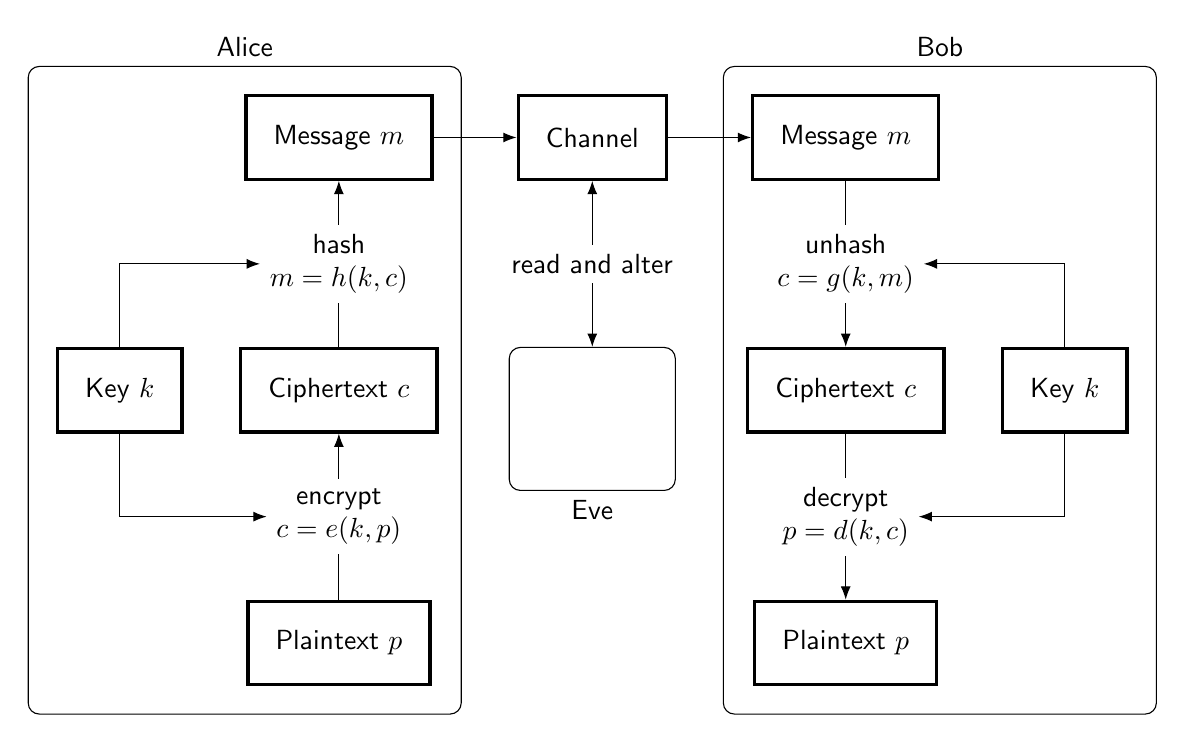
\begin{tikzpicture}[
		node distance=6em,
		action/.style={midway, fill=white, align=center},
		arrow/.style={-Latex},
		block/.style={draw, very thick, fill=white, minimum height=7ex, minimum width=3.5, inner xsep=1em},
		superblock/.style={draw, rounded corners, inner sep=1em},
	]
		\coordinate (in) at (0,0);
		\node [block, above=of in] (plain a) {\textsf{Plaintext} $p$};
		\node [block, above=of plain a] (cipher a) {\textsf{Ciphertext} $c$};
		\node [block, left=2em of cipher a] (key a) {\textsf{Key} $k$};
		\node [block, above=of cipher a] (message a) {\textsf{Message} $m$};
		\node [block, right=3em of message a)] (channel) {\textsf{Channel}};
		\node [block, right=3em of channel] (message b) {\textsf{Message} $m$};
		\node [block, below=of message b] (cipher b) {\textsf{Ciphertext} $c$};
		\node [block, right=2em of cipher b] (key b) {\textsf{Key} $k$};
		\node [block, below=of cipher b] (plain b) {\textsf{Plaintext} $p$};
		\coordinate[below=of plain b] (out);
		
		\node [superblock, label=\textsf{Alice}, fit=(plain a) (key a) (message a)] {};
		\node [superblock, label={below:\textsf{Eve}}, below=of channel, minimum width=6em, minimum height=12ex]  (eve) {};
		\node [superblock, label=\textsf{Bob}, fit=(plain b) (key b) (message b)] {};
		
		\draw[arrow] (plain a) -- (cipher a) node[action] (enc) {\textsf{encrypt}\\$c=e(k,p)$};
		\draw[arrow] (cipher a) -- (message a) node[action] (hash) {\textsf{hash}\\$m=h(k,c)$};
		\draw[arrow] (message a) -- (channel);
		\draw[arrow] (channel) -- (message b);	
		\draw[arrow] (message b) -- (cipher b) node[action] (unhash) {\textsf{unhash}\\$c=g(k,m)$};		
		\draw[arrow] (cipher b) -- (plain b) node[action] (dec) {\textsf{decrypt}\\$p=d(k,c)$};
		
		\draw[arrow] (key a) -- (key a|-enc) -- (enc);
		\draw[arrow] (key a) -- (key a|-hash) -- (hash);
		\draw[arrow] (key b) -- (key b|-dec) -- (dec);
		\draw[arrow] (key b) -- (key b|-unhash) -- (unhash);
		
		\draw [Latex-Latex] (eve) -- (channel) node[action] {\textsf{read and alter}};
	\end{tikzpicture}
\end{document}
